\documentclass[10pt,table,xcolor=dvipsnames]{beamer}
\usepackage[utf8]{luainputenc}
\usepackage[ngerman]{babel}


%\usetheme[block=fill]{m}                     % Use metropolis theme
\usepackage{beamerthemeuzl-conference}

\usepackage{Alegreya,AlegreyaSans}

\logo{
\includegraphics[scale=.62]{uzl-logo-ITCS.pdf}}
\usepackage{amsmath}
\DeclareMathOperator*{\argmin}{arg\,min}
\usepackage{nicefrac}
\usepackage{algorithm}
\usepackage{dsfont}
\usepackage{subfig}
\usepackage{mathtools}
\usepackage{graphicx}
\usepackage{mathpazo} 
\usepackage{tikz}

% Finn
\usepackage{xspace}
\usepackage{float}
\usepackage{subfig}
\usepackage{color, colortbl}
\definecolor{uzlred}{HTML}{BF0000}
\definecolor{uzlgreen}{HTML}{008000}
\definecolor{uzlpurple}{HTML}{700080}
\newcommand{\highlightrow}{\rowcolor{Ozeangruen!5}}

% mine
\usepackage{mathtools}
\usepackage{algpseudocode}
\usetikzlibrary{positioning,shapes,snakes,automata,shadows,arrows,trees,fit}
\usepackage{tikz-qtree}
\usepackage{transparent}
\setbeamercovered{transparent}
\tikzstyle{gray}  = [thick, color=gray, circle, draw]
\tikzstyle{red}   = [thick, color=red, circle, draw]
\tikzstyle{blue}  = [thick, color=blue, circle, draw]
\tikzstyle{green} = [thick, color=green, circle, draw]
\usepackage{wasysym}

\newtheorem{lem}{Lemma}

\title{Algorithmen für das Moving-Target Travelling Salesman Problem}
%\subtitle{}
\author{Felix Greuling}
\date{27.01.2019}


\begin{document}
\maketitle


%\iffalse
\begin{frame}{Überblick}
\tableofcontents[hideallsubsections]
\end{frame}

\AtBeginSection[]
{
  \begin{frame}
    \frametitle{Überblick}
    \tableofcontents[currentsection, hideallsubsections]
  \end{frame}
}
%\fi

\AtBeginSection[]{
  \begin{frame}[noframenumbering]
  \vfill
  \centering
  \begin{beamercolorbox}[sep=8pt,center,shadow=true,rounded=true]{title}
    \usebeamerfont{title}\insertsectionhead\par%
  \end{beamercolorbox}
  \vfill
  \end{frame}
}



\section{Einleitung}
\begin{frame}{Einleitung}
Travelling Salesman Problem (TSP)
\begin{itemize}
\item
Optimierungsproblem aus der Kombinatorik \pause
\item
Reihenfolge an Zielen, sodass die Tourzeit minimal ist \pause
\item
Tour startet und endet im selben Ziel \pause
\item
NP-vollständig
\end{itemize}
\end{frame}

\begin{frame}{Einleitung}
\begin{center}
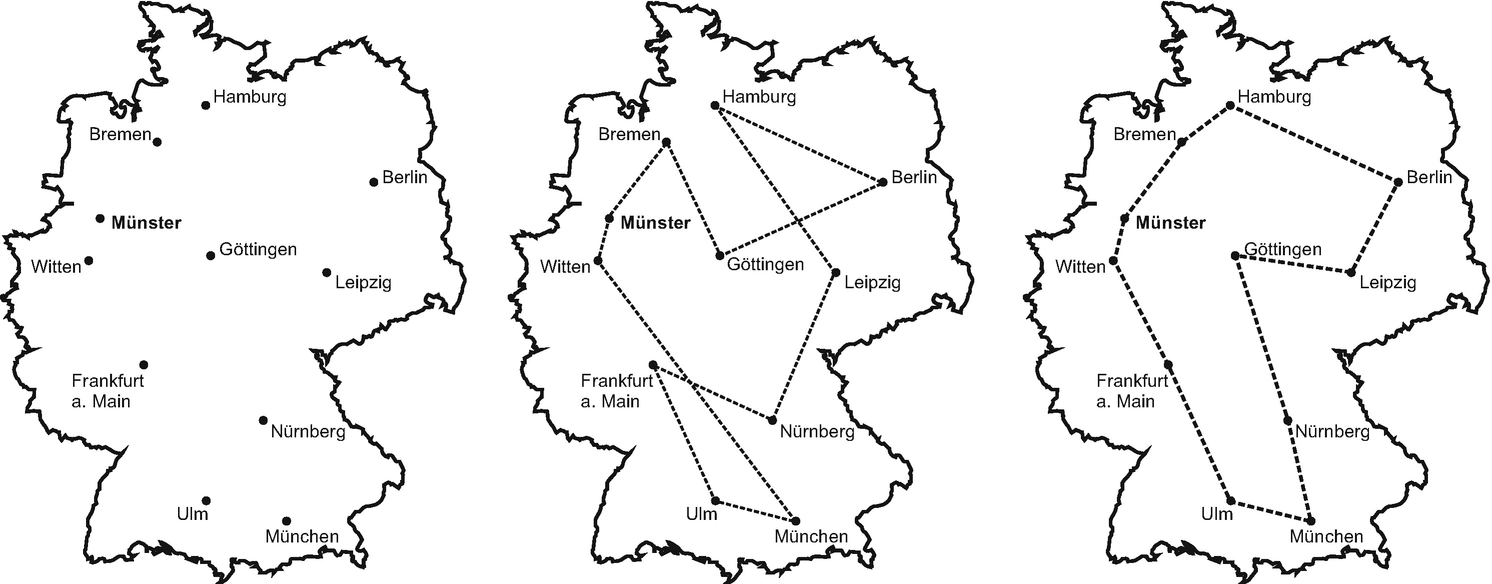
\includegraphics[scale=0.8]{Images/TSP.png}\\~\\
\end{center}
\end{frame}

\begin{frame}{Einleitung}
Moving-Target-TSP (MT-TSP)
\begin{itemize}
\item
Im Jahre 1998 von Helvig et al. erwähnt \pause
\item
Ziele sind nun nicht mehr stationär \pause
\item
Problematik bleibt die selbe
\end{itemize}

\end{frame}

\begin{frame}{Einleitung}
\centering
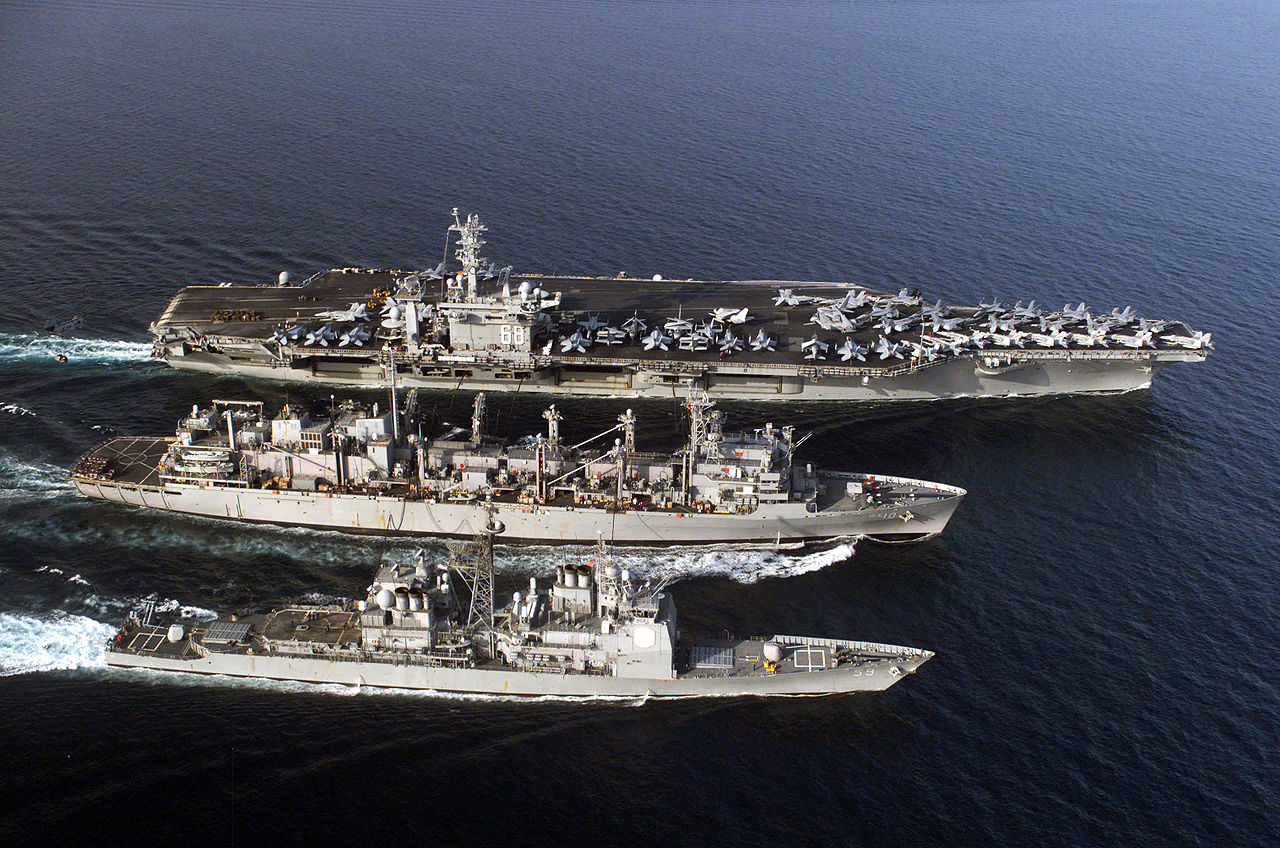
\includegraphics[scale=0.8]{Images/Versorgungsschiff.jpg}
\end{frame}

\section{Grundlagen}
%\begin{frame}{MT-TSP}
%Formal haben Helvig et al. das Problem wie folgt definiert:\\~\\
%\begin{quote}
%The moving-target traveling salesman problem: Given a set $S = \{s_1, \dots , s_n\}$ of \emph{targets}, each $s_i$ moving at constant velocity $\overrightarrow{v_i}$ from an initial position $p_i$, and given a \emph{pursuer} starting at the origin and having maximum speed $v>|\overrightarrow{v_i}|$, find the fastest tour starting (and ending) at the origin, which intercepts all targets.
%\end{quote}
%\end{frame}

\begin{frame}{MT-TSP}
\begin{itemize}
\item Ziele
\begin{align*}
Z = (z_1, ..., z_n)
\end{align*} 
\item Startpositionen 
\begin{align*}
P = (p_1, ..., p_n)
\end{align*} 
\item Geschwindigkeiten
\begin{align*}
V = (v_1, ..., v_n)
\end{align*} 
\item Verfolger
\begin{align*}
\kappa = (p_\kappa,v_\kappa)~~~~
\end{align*}
\end{itemize}
\end{frame}

\begin{frame}{MT-TSP in einer Dimension}
\begin{figure} 
\centering
\scalebox{0.8}{
\begin{tikzpicture}
\coordinate (a) at (-5,0) node[below=0.1cm of a]{-1000};
\coordinate (b) at (-1,0) node[below=0.1cm of b]{-1};
\coordinate (c) at (0,0) node[below=0.1cm of c]{0};
\coordinate (d) at (1,0) node[below=0.1cm of d]{1};
\coordinate (e) at (5,0) node[below=0.1cm of e]{1000};
\coordinate (f) at (-6,0) node[below=0.1cm of f, xshift=3.0cm]{[...]};
\coordinate (g) at (6,0) node[below=0.1cm of g, xshift=-3.0cm]{[...]};
% Geschwindigkeiten
\node[above of=a, xshift=-0.1cm, yshift=0.1cm] {$-1$};
\node[above of=b, xshift=-0.3cm, yshift=0.1cm] {$-8$};
\node[above of=d, xshift=0.3cm, yshift=0.1cm] {$8$};
\node[above of=e, xshift=0.1cm, yshift=0.1cm] {$1$};
\fill (a) circle (2.5pt);
\fill (b) circle (2.5pt);
\fill (d) circle (2.5pt);
\fill (e) circle (2.5pt);
\draw (f)--(a)--(b)--(c)--(d)--(e)--(g);
% links 1.
\coordinate (aa) at (-5,0.8);
\draw (a) -- (aa);
\draw (-5,0.8) -- (-5.2,0.8);
\draw (-5.2,0.9) -- (-5.4,0.8) -- (-5.2,0.7) -- cycle;
% links 2.
\coordinate (bb) at (-1,0.8);
\draw (b) -- (bb);
\draw (-1,0.8) -- (-1.7,0.8);
\draw (-1.7,0.9) -- (-1.9,0.8) -- (-1.7,0.7) -- cycle;
% mitte
\draw (0,2) -- (0,1.5) -- (0.4,1.75) -- cycle;
\coordinate (cc) at (0,2);
\draw (c) -- (cc);
% rechts 2.
\coordinate (dd) at (1,0.8);
\draw (d) -- (dd);
\draw (1,0.8) -- (1.7,0.8);
\draw (1.7,0.9) -- (1.9,0.8) -- (1.7,0.7) -- cycle;
% rechts 1.
\coordinate (ee) at (5,0.8);
\draw (e) -- (ee);
\draw (5,0.8) -- (5.2,0.8);
\draw (5.2,0.9) -- (5.4,0.8) -- (5.2,0.7) -- cycle;
\end{tikzpicture}} 
\caption{Eindimensionaler Fall mit jeweils zwei Zielen auf beiden Seiten des Ursprungs.}
\end{figure} 
\begin{itemize}
\item<1,2,3> Ziele $Z=\{(-1000,-1),(-1,-8),(1,8),(1000,1)\}$
\item<1,2,3> Verfolger $\kappa=(0,10)$
\item<2,3> Betrachten für optimale Strategie Wendepunkte
\item<3> $Left=\{(-1,-8),(-1000,-1)\}$ 
\item<3> $Right=\{(1,8),(1000,1)\}$
\end{itemize}

\end{frame}

\begin{frame}{MT-TSP in einer Dimension}
\begin{itemize}
\item $Left=\{(-1,-8),(-1000,-1)\}$ 
\item $Right=\{(1,8),(1000,1)\}$
\item $A=(s_k,s_f)$
\end{itemize}
\pause
\centering
\scalebox{0.8}{\parbox{.5\linewidth}{
\begin{align*}
A_0&=\emptyset\\
A_1&=\{(-1, -8), (1, 8)\} &\text{Index-Summenwert}=0\\
A_2&=\{(1, 8), (-1, -8)\} &\text{Index-Summenwert}=0\\ 
A_3&=\{(-1, -8), (1000, 1)\} &\text{Index-Summenwert}=1~\\
A_4&=\{(1000, 1), (-1, -8)\} &\text{Index-Summenwert}=1~\\
A_5&=\{(-1000, -1), (1, 8)\} &\text{Index-Summenwert}=1~\\
A_6&=\{(1, 8), (-1000, -1)\} &\text{Index-Summenwert}=1~\\
A_7&=\{(-1000, -1), (1000, 1)\} &\text{Index-Summenwert}=2~\\
A_8&=\{(1000, 1), (-1000, -1)\} &\text{Index-Summenwert}=2~\\
A_{9}&=\emptyset
\end{align*}
}}
\end{frame}

\begin{frame}{MT-TSP in einer Dimension}
\begin{figure}
\centering
\scalebox{0.7}{
\begin{tikzpicture}[->, thick]
\node[state] (A0) {$A_0$};
\node[state, above right = of A0, yshift=+1.1cm, xshift=0.2cm] (A1) {$A_1$};
\node[state, below right = of A0, yshift=-1.1cm, xshift=0.2cm] (A2) {$A_2$};
\node[state, above right = of A1, yshift=-0.3cm, xshift=0.6cm] (A5) {$A_5$};
\node[state, below right = of A1, yshift=+0.3cm, xshift=0.6cm] (A6) {$A_6$};
\node[state, above right = of A2, yshift=-0.3cm, xshift=0.6cm] (A3) {$A_3$};
\node[state, below right = of A2, yshift=+0.3cm, xshift=0.6cm] (A4) {$A_4$};
\node[state, right = of A6, xshift=0.6cm] (A7) {$A_7$};
\node[state, right = of A3, xshift=0.6cm] (A8) {$A_8$};
\node[state, right = of A0, xshift = 8cm] (A9) {$A_9$};
\end{tikzpicture}}
\caption{Zustände in aufsteigender Reihenfolge der Summenindizes.}
\end{figure}
\end{frame}

\begin{frame}[noframenumbering]{MT-TSP in einer Dimension}
\begin{figure}
\centering
\scalebox{0.7}{
\begin{tikzpicture}[->, thick]
\node[state] (A0) {$A_0$};
\node[state, above right = of A0, yshift=+1.1cm, xshift=0.2cm] (A1) {$A_1$};
\node[state, below right = of A0, yshift=-1.1cm, xshift=0.2cm] (A2) {$A_2$};
\node[state, above right = of A1, yshift=-0.3cm, xshift=0.6cm] (A5) {$A_5$};
\node[state, below right = of A1, yshift=+0.3cm, xshift=0.6cm] (A6) {$A_6$};
\node[state, above right = of A2, yshift=-0.3cm, xshift=0.6cm] (A3) {$A_3$};
\node[state, below right = of A2, yshift=+0.3cm, xshift=0.6cm] (A4) {$A_4$};
\node[state, right = of A6, xshift=0.6cm] (A7) {$A_7$};
\node[state, right = of A3, xshift=0.6cm] (A8) {$A_8$};
\node[state, right = of A0, xshift = 8cm] (A9) {$A_9$};

\path (A0) edge [bend left] (A1) node[xshift=0.8cm, yshift=1.5cm] {$\tau_{left}$};
\path (A0) edge [bend right] (A2) node[xshift=0.8cm, yshift=-1.5cm] {$\tau_{right}$};

\path (A1) edge [bend left] (A5) node[xshift=1.1cm, yshift=0.9cm] {$\tau_{left}$};
\path (A1) edge [bend right] (A6) node[xshift=1.1cm, yshift=-0.9cm] {$\tau_{right}$};
\path (A2) edge [bend left] (A3) node[xshift=1.1cm, yshift=0.8cm] {$\tau_{right}$};
\path (A2) edge [bend right] (A4) node[xshift=1.1cm, yshift=-0.9cm] {$\tau_{left}$};

\path (A5) edge [bend left] (A9) node[xshift=3.8cm, yshift=-0.9cm] {$\tau_{final}$};
\path (A4) edge [bend right] (A9) node[xshift=3.8cm, yshift=0.8cm] {$\tau_{final}$};

\path (A6) edge (A7) node[xshift=1.3cm, yshift=+0.2cm] {$\tau_{left}$};
\path (A6) edge (A8) node[xshift=1.0cm, yshift=-0.5cm] {$\tau_{right}$};
\path (A3) edge (A7) node[xshift=1.0cm, yshift=+0.5cm] {$\tau_{left}$};
\path (A3) edge (A8) node[xshift=1.3cm, yshift=-0.2cm] {$\tau_{right}$};

\path (A7) edge (A9) node[xshift=1.1cm, yshift=-0.8cm] {$\tau_{final}$};
\path (A8) edge (A9) node[xshift=1.1cm, yshift=+0.8cm] {$\tau_{final}$};
\end{tikzpicture}}
\caption{Zustände in aufsteigender Reihenfolge der Summenindizes.}
\end{figure}
\end{frame}

\section{Zwei-orthogonale-Achsen im MT-TSP}
\begin{frame}{Zwei-orthogonale-Achsen im MT-TSP}
\begin{itemize}
\item
Neue Modifikation mit zusätzlicher Achse \pause
\item
Ziele und Verfolger können sich ausschließlich auf dieser bewegen \pause
\item
Dem Verfolger ist es möglich, die Achse zu wechseln 
\end{itemize}
\end{frame}

\subsection{Theoretische Grundlagen}
\begin{frame}{Theoretische Grundlagen}
\begin{block}{Lemma 1}
In jeder optimalen Tour bei zwei orthogonalen Achsen im MT-TSP muss sich der Verfolger mit seiner  maximalen Geschwindigkeit bewegen.
\end{block}
\begin{block}{Lemma 2}
In jeder optimalen Tour bei zwei orthogonalen Achsen im MT-TSP gelten für den Verfolger folgende Eigenschaften:
\begin{itemize}
\item
Bewegt sich der Verfolger wegführend vom Ursprung, ändert dieser erst seine Richtung, sofern er das schnellste Ziel in seiner Richtung abgefangen hat.
\item
Bewegt sich der Verfolger in Richtung des Ursprungs, ändert dieser solange nicht seine Richtung, bis er den Ursprung erreicht hat.
\end{itemize}
\end{block}
\end{frame}


\subsection{Heuristiken}
\begin{frame}{Problem}
\begin{figure}
\centering
\scalebox{0.7}{
\begin{tikzpicture}
\coordinate (o) at (0,0) ;
\coordinate (l) at (-6,0);
\coordinate (r) at (6,0); 
\coordinate (b) at (0,-3); 
\coordinate (t) at (0,6); 
\draw (l)--(r) (b)--(t);
% target 1 left ((-10,0),5)
\coordinate (l1) at (-2,0) node[below=0.1cm of l1]{-10};
\fill (l1) circle (2.5pt);
\coordinate (l1a) at (-2,0.8) node[above=0.1cm of l1a, xshift=0.1cm]{5};
\draw (l1) -- (l1a) -- (-1.7,0.8);
\draw (-1.7,0.9) -- (-1.5,0.8) -- (-1.7,0.7) -- cycle;
% target 2 left ((-15,0),-7)
\coordinate (l2) at (-3,0) node[below=0.1cm of l2]{-15};
\fill (l2) circle (2.5pt);
\coordinate (l2a) at (-3,0.8) node[above=0.1cm of l2a, xshift=-0.2cm]{-7};
\draw (l2) -- (l2a) -- (-3.4,0.8);
\draw (-3.4,0.9) -- (-3.6,0.8) -- (-3.4,0.7) -- cycle;
% target 3 top ((25,1),13)
\coordinate (l3) at (0,4.5) node[left=0.1cm of l3]{25};
\fill (l3) circle (2.5pt);
\coordinate (l3a) at (0.8,4.5) node[right=0.1cm of l3a, yshift=0.4cm]{13};
\draw (l3) -- (l3a) -- (0.8,5.2);
\draw (0.7,5.2) -- (0.8,5.4) -- (0.9,5.2) -- cycle;
\end{tikzpicture}
} \caption{Bei zwei-orthogonale-Achsen-Fällen können Ziele den Ursprung überqueren, während der Verfolger auf einer Achse ein Ziel verfolgt.}
\end{figure}
\end{frame}

%\begin{frame}[noframenumbering]{Problem}
%\begin{figure}
%\centering
%\scalebox{0.7}{
%\begin{tikzpicture}
%\coordinate (o) at (0,0) ;
%\coordinate (l) at (-6,0);
%\coordinate (r) at (6,0); 
%\coordinate (b) at (0,-3); 
%\coordinate (t) at (0,6); 
%\draw (l)--(r) (b)--(t);
%% target 1 left ((-10,0),5)
%\coordinate (l1) at (-2,0) node[below=0.1cm of l1]{-10};
%\fill (l1) circle (2.5pt);
%\coordinate (l1a) at (-2,0.8) node[above=0.1cm of l1a, xshift=0.1cm]{5};
%\draw (l1) -- (l1a) -- (-1.7,0.8);
%\draw (-1.7,0.9) -- (-1.5,0.8) -- (-1.7,0.7) -- cycle;
%% target 2 left ((-15,0),-7)
%\coordinate (l2) at (-3,0) node[below=0.1cm of l2]{-15};
%\fill (l2) circle (2.5pt);
%\coordinate (l2a) at (-3,0.8) node[above=0.1cm of l2a, xshift=-0.2cm]{-7};
%\draw (l2) -- (l2a) -- (-3.4,0.8);
%\draw (-3.4,0.9) -- (-3.6,0.8) -- (-3.4,0.7) -- cycle;
%% target 3 top ((25,1),13)
%\coordinate (l3) at (0,4.5) node[left=0.1cm of l3]{25};
%\fill (l3) circle (2.5pt);
%\coordinate (l3a) at (0.8,4.5) node[right=0.1cm of l3a, yshift=0.4cm]{13};
%\draw (l3) -- (l3a) -- (0.8,5.2);
%\draw (0.7,5.2) -- (0.8,5.4) -- (0.9,5.2) -- cycle;
%% target 4 right ((20,0),4)
%\coordinate (r1) at (4,0) node[below=0.1cm of r1]{20};
%\fill[red] (r1) circle (2.5pt);
%\coordinate (rra) at (4,0.8) node[above=0.1cm of rra, xshift=0.1cm]{4};
%\draw[red]  (r1) -- (rra) -- (4.3,0.8);
%\draw[red]  (4.3,0.9) -- (4.5,0.8) -- (4.3,0.7) -- cycle;
%\end{tikzpicture}
%} \caption{Bei zwei-orthogonale-Achsen-Fällen können Ziele den Ursprung überqueren, während der Verfolger auf einer Achse ein Ziel verfolgt.}
%\end{figure}
%\end{frame}

\begin{frame}{Prioritätsansatz}
\small
\begin{itemize}
\item 
Gewichte
\begin{align*}
\omega = (w_1, w_2 ,w_3)
\end{align*}\pause
\item
Geschwindigkeitsfaktor
\begin{align*}
\varphi_1(z_i, w_1) = \frac{|v_i|}{v_{\kappa}}\cdot w_1
\end{align*}\pause
\item
Positionsfaktor
\begin{align*}
\varphi_2(z_i, w_2) = \frac{|p_i|}{v_{\kappa}}\cdot a \cdot w_2
\end{align*}\pause
\item
Distanzfaktor
\begin{align*}
\varphi_3(z_i, w_3) = \bigg\vert\frac{\|p_{verfolger},p_i\|_1}{v_{\kappa}-v_i}\bigg\vert \cdot w_3
\end{align*}\pause
\item
Priorität
\begin{align*}
\alpha_i(z_i, \omega) := \varphi_1(z_i,w_1) + \varphi_2(z_i,w_2) - \varphi_3(z_i,w_3)
\end{align*}
\end{itemize}
\normalsize
\end{frame}

\begin{frame}{Prioritätsansatz}
\begin{itemize}
\item
In jeder Iteration des Algorithmus wird
\begin{itemize}
\item
die Priorität jedes Ziels berechnet
\item
die Position von jedem Ziel aktualisiert
\item
geprüft, ob Ziele zwischen dem betrachteten und dem vorherigen Ziel abgefangen wurden
\end{itemize}
\pause
\item
garantiert keine optimalen Ergebnisse
\pause
\item
$\mathcal{O}(n^2)$
\end{itemize}
\end{frame}

\begin{frame}{Brute-Force-Ansatz}
\begin{figure}
\centering
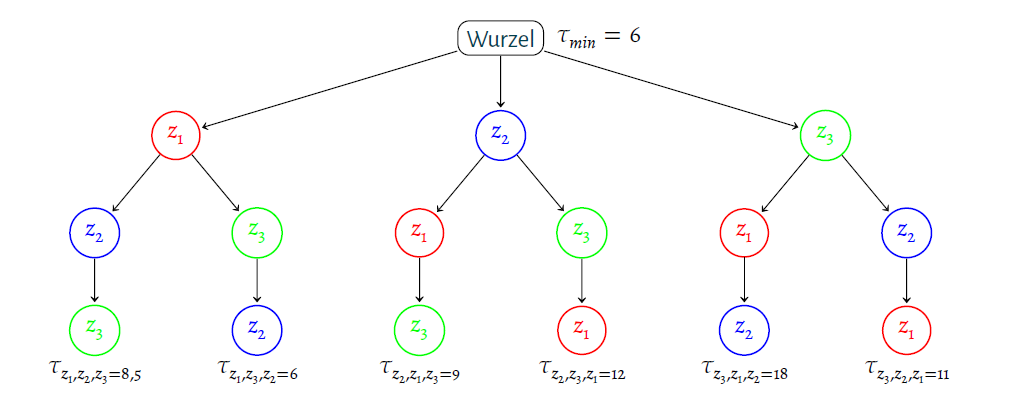
\includegraphics[scale=0.3]{Images/BF1.png}
\caption{Brute-Force-Ansatz bei $n=3$ Zielen.}
\end{figure}
\end{frame}

\begin{frame}[noframenumbering]{Brute-Force-Ansatz}
\begin{figure}
\centering
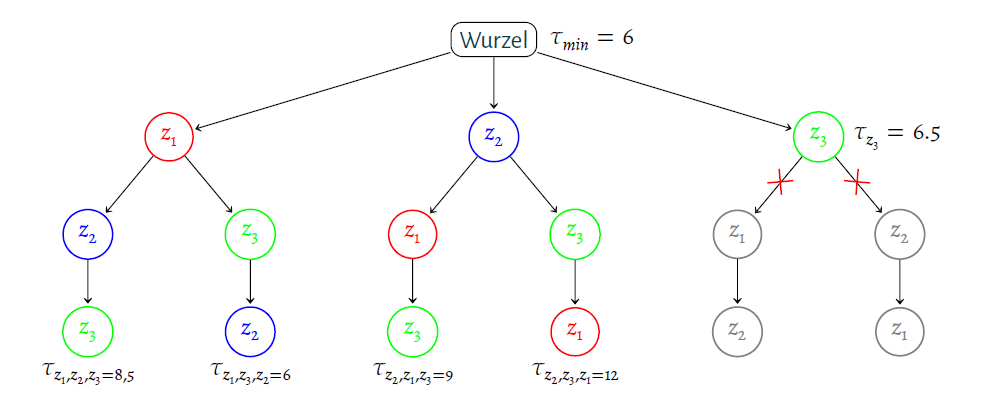
\includegraphics[scale=0.3]{Images/BF2.png}
\caption{Brute-Force-Ansatz bei $n=3$ Zielen.}
\end{figure}
\end{frame}

\section{Ergebnisse}
\begin{frame}{Durchschnittliche Laufzeit des 1D-Algorithmus}
\centering
\begin{figure}
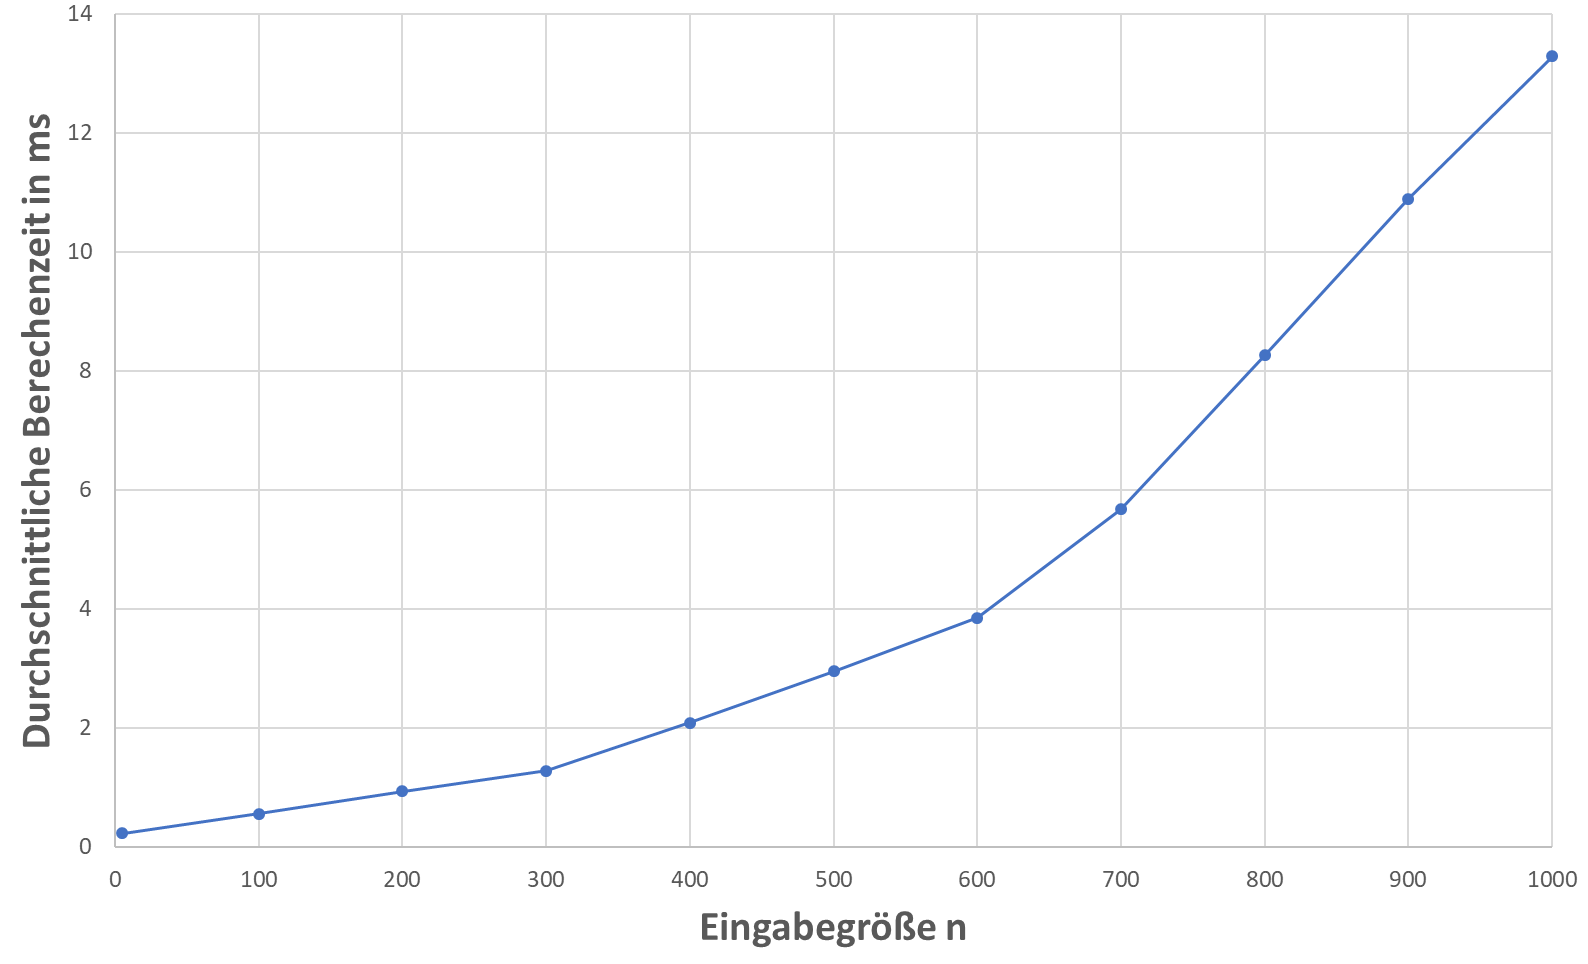
\includegraphics[scale=0.15]{Images/Exp1D.png}
\caption{Berechenzeit der optimalen Tour bei bis zu $1.000$ Zielen und $v_{\kappa}=40$.}
\end{figure}
\end{frame}

\begin{frame}{Brute-Force-Algorithmus mit unterschiedlichen Eingabegrößen}
\centering
\begin{table}
\scalebox{0.70}{
\begin{tabular}{ccccccc} 
\hline
$n$ &Instanzen&$\diameter$betr. Knoten & $\diameter$Anteil Knoten & $\diameter$Schnitte & $\diameter$ber. Blätter & Fails\\ \hline
1& 10.000& ~~~~~~~~~~~1,00& 1,000000& ~~~~~~~~0,00& ~~~~1,00& ~0 \\
2& 10.000& ~~~~~~~~~~~3,75& 0,939151& ~~~~~~~~0,24& ~~~~1,57& ~0 \\
3& 10.000& ~~~~~~~~~~11,75& 0,783513& ~~~~~~~~0,95& ~~~~3,14& ~0 \\
4& 10.000& ~~~~~~~~~~37,81& 0,590758& ~~~~~~~~3,22& ~~~~6,71& ~0 \\
5& 10.000& ~~~~~~~~~130,44& 0,401344& ~~~~~~~11,87& ~~~15,02& ~0 \\
6& 10.000& ~~~~~~~~~471,76& 0,241184& ~~~~~~~47,23& ~~~32,46& ~0 \\
7& 10.000& ~~~~~1.819,94& 0,132852& ~~~~~~194,96& ~~~70,33& ~0 \\
8& 10.000& ~~~~~7.353,01& 0,067090& ~~~~~~852,13& ~~150,30& ~0 \\
9& 10.000& ~~~~31.426,98& 0,031860& ~~~~3.833,61& ~~313,76& ~0 \\
10&~1.000& ~~~140.342,54& 0,014228& ~~~18.169,79& ~~620,86& ~0 \\
11&~1.000& ~~~650.570,40& 0,005996& ~~~88.862,13& 1.304,56& ~0 \\
12&~~~100& 3.562.601,51& 0,002736& ~~457.589,77& 3.246,11& ~0 \\
13&~~~100& 8.184.931,87& 0,000484& 1.523.396,29& 4.303,92& 22\\
14&~~~~10& 5.033.246,67& 0,000021& 1.147.070,33& 2.025,67& ~7 \\ \hline
\end{tabular}}
\caption{Beschneidungen im Suchbaum des Brute-Force-Algorithmus bei einer Eingabe von $1\leq n\leq 14$ Zielen und $v_{\kappa}=40$.}
\end{table}
\end{frame}

\begin{frame}{Güte des Prioritäts-Algorithmus}
\begin{table}
\centering
\scalebox{0.8}{
\begin{tabular}{ccccccc} 
\hline
\emph{$n$} & \emph{Instanzen}& \emph{$max\{v_i\}$} & \emph{$\diameter$Güte} & \emph{max Güte} & \emph{opt. Touren} & \emph{Anteil opt.}\\ \hline
~8& 10.000& 20& 1,10& ~~2,59& 6313& 0,63 \\
~8& 10.000& 40& 1,41& ~11,93& 3341& 0,33 \\
~8& 10.000& 60& 3,53& 328,88& 1390& 0,14 \\
10& ~~1.000& 20& 1,14& ~~2,15& ~518& 0,52 \\
10& ~~1.000& 40& 1,54& ~~9,22& ~220& 0,22 \\
10& ~~1.000& 60& 5,32& 282,26& ~~83& 0,08 \\
12& ~~~~~~100& 20& 1,16& ~~2,31& ~~43& 0,43 \\
12& ~~~~~~100& 40& 1,56& ~~4,79& ~~12& 0,12 \\
12& ~~~~~~100& 60& 5,30& ~82,29& ~~~5& 0,05 \\ \hline
\end{tabular}}
\caption{Güte des Prioritäts-Algorithmus bei $\omega=(87,34,31)$ und $v_{\kappa}=61$.}
\label{tab:ExpGüte}
\end{table}
\end{frame}

\section{Zusammenfassung und Ausblick}
\begin{frame}{Zusammenfassung}
\begin{itemize}
\item
1D-Algorithmus auch bei großen Instanzen effizient 
\pause
\item
Prioritätsalgorithmus abhängig von den gewählten Gewichten 
\pause
\item
Brute-Force-Algorithmus effizient, sofern schnell ein kleines $\tau_{min}$ gefunden wird.
\end{itemize}
\end{frame}

\begin{frame}{Ausblick}
\begin{itemize}
\item
Weiterhin optimale Heuristik mit polynomieller Laufzeit gesucht 
\pause
\item
$k$-Achsen im MT-TSP
\end{itemize}
\end{frame}


\nocite{*}
\appendix
\begin{frame}[noframenumbering, plain]
\Large\center
Danke für Ihre Aufmerksamkeit!
\end{frame}


\begin{frame}[noframenumbering]{References} 
	\bibliographystyle{amsalpha}
	\bibliography{lit}
\end{frame}

%-----------------------------------------------------------------------------------

\begin{frame}[allowframebreaks, noframenumbering]{Lemmata}
\scriptsize
\begin{lem}
\label{lem:1}
In jeder optimalen Tour bei zwei orthogonalen Achsen im MT-TSP muss sich der Verfolger mit seiner  maximalen Geschwindigkeit bewegen.
\end{lem}
 
\framebreak 
 
\begin{proof}
Der Beweis basiert darauf, dass in jedem Fall eine Reduzierung auf den Beweis von \cite{helvig} vorgenommen wird. Nehmen dafür eine Fallunterscheidung vor:
\begin{enumerate}
\item Das nächste Ziel des Verfolgers liegt auf der selben Achse:

Mit dem Beweis für 1D-Fälle in \cite{helvig} gilt dies auch für diesen Fall.\\

\item Das nächste Ziel des Verfolgers bewegt sich auf der anderen Achse: 

Wir nehmen für einen Widerspruch an, der Verfolger bewegt sich mit $v < v_{\kappa}$. Dies ist äquivalent dazu, dass der Verfolger an seiner aktuellen Position eine Zeit $\tau$ wartet und sich dann mit $v_{\kappa}$ weiterbewegt, um dann das nächste Ziel $z$ einzuholen. Dabei befindet sich $z$ auf der anderen Achse. Nach der Wartezeit erreicht der Verfolger an Zeitpunkt $t_1$ den Ursprung und holt das Ziel $z$ an der Position $p$ zum Zeitpunkt $t_2$ ein. 

Nehmen nun an, dass der Verfolger sich direkt zum Mittelpunkt bewegt. Bis zum Eintreffen des Zeitpunktes $t_1$ wartet der Verfolger nun wieder die Zeit $\tau$. Das Ziel $z$ wird nun zum selben Zeitpunkt $t_2$ bei $p$ erreicht, wie im vorherigen Szenario. Dies wird nun fortgeführt, indem der Verfolger nicht im Ursprung wartet, sondern von diesem aus $p$ direkt erreicht. Bis zum Zeitpunkt $t_2$ wird nun wieder für die Dauer von $\tau$ gewartet. Außerdem kann der Verfolger schon zu einem Zeitpunkt $t_1 \leq t_{s} \leq t_2$ abfangen, sofern sich $z$ vom Verfolger wegbewegt. 

Werden die Wartezeiten nun jeweils auch für alle restlichen Ziele der Tour hinten angehängt, resultiert dies letztendlich in Wartezeit am Ende der Tour, was offensichtlich nicht optimal ist. Dieser Fall ist demnach nur eine Erweiterung des 1D-Fall-Beweises um den Ursprung zwischen Zielen, die auf unterschiedlichen Achsen liegen. 
\end{enumerate}
In jedem der Fälle wird eine Wartezeit erzeugt, welche an das Ende der Tour verschoben werden kann. Somit ist die Tour offensichtlich nicht mehr optimal. Der Verfolger bewegt sich also zu jeder Zeit mit $v_{\kappa}$.
\end{proof}

\framebreak

\begin{lem}
\label{lem:2}
In jeder optimalen Tour bei zwei orthogonalen Achsen im MT-TSP gelten für den Verfolger folgende Eigenschaften:
\begin{itemize}
\item
Bewegt sich der Verfolger wegführend vom Ursprung, ändert dieser erst seine Richtung, sofern er das schnellste Ziel in seiner Richtung abgefangen hat.
\item
Bewegt sich der Verfolger in Richtung des Ursprungs, ändert dieser solange nicht seine Richtung, bis er den Ursprung erreicht hat.
\item
\textcolor{red}{Der Verfolger befindet sich im Ursprung, kann sich dieser nicht in die Richtung bewegen, aus die er gerade kommt.}
\end{itemize}
\end{lem}

\framebreak

\textcolor{TealBlue}{Beweis.}\\
Für den Beweis des Lemmas müssen beide Eigenschaften bewiesen werden. Fallunterscheidung:
\begin{itemize}
\item[1.]
Der Verfolger bewegt sich wegführend vom Ursprung in Richtung des schnellsten Ziels $z_1$: 

Der Verfolger kann sich dabei auf einer beliebigen Position der vier Seiten des Ursprungs\footnote{Die Position kann sich ebenfalls auf dem Ursprung selbst befinden.} zum Zeitpunkt $t_1$ befinden. Der Beweis für diesen Fall ist ähnlich zu dem Beweis für Wendepunkte aus \cite{helvig}.

Wir nehmen für einen Widerspruch an, dass der Verfolger in einer optimalen Tour seine Richtung zum Zeitpunkt $t_2$ ändert, bevor $z_1$ abgefangen wurde. Damit gibt es ein kleines $\delta>0$, sodass in dem Zeitraum zwischen $t_2-\delta$ und $t_2+\delta$ der Verfolger nur zum Zeitpunkt $t_2$ seine Richtung ändert. Wir nehmen als alternative Tour an, dass der Verfolger zum Zeitpunkt $t_2-\delta$ anhält und bis $t_2+\delta$ im selben Punkt $p$ wartet. Anschließend setzt er die ursprüngliche Tour fort. Jegliche Ziele\footnote{Ziele, die auf der Seite des Ursprungs gestartet sind.} befinden sich in dem Zeitraum von $t_2-\delta$ bis $t_2+\delta$ zwischen $p$ und $z_1$ und sind nach Definition langsamer, als $z_1$, sodass diese $z_1$ nicht überholen können. Mit der Wartezeit wird also die Tourzeit nicht reduziert.

Betrachten als Ausnahme das Ziel $z_2$ von der anderen Seite des Ursprungs. Im Gegensatz zum eindimensionalen Fall kann ein solches Ziel alle Ziele auf der anderen Seite des Ursprungs überholen. Dabei befindet sich  $z_2$ zum Zeitpunkt $t_1$ zwischen dem Ursprung und $p$. Sei $z_2$ schneller als $z_1$. Somit erreicht der Verfolger $z_2$ zwischen $p$ und $z_1$. Allerdings wird damit die Tourzeit ebenfalls nicht verbessert, da $z_2$ sowieso auf dem Rückweg zum Ursprung abgefangen wird. 

Selbst wenn der Verfolger vor $z_1$ die Richtung ändert, um ein Ziel auf einer der anderen drei Seiten abzufangen, hat der Verfolger in der vorherigen Zeit nicht das Ziel $z_1$ verfolgt und nur Ziele abgefangen, die sich auf dem Weg dorthin befanden. Demnach führt die Zeit, die nicht für das Verfolgen des schnellsten Ziels aufgewendet wurde, zu einer Wartezeit an einer Position. Somit wäre die Tour nach Lemma \ref{lem:1} nicht optimal.
\end{itemize}

\framebreak

\begin{itemize}
\item[2.]
Der Verfolger hat soeben das schnellste Ziel auf einer Achse abgefangen und bewegt sich nun zum Ursprung:

Dieses Szenario gilt ebenfalls für alle vier Seiten des Ursprungs. Dabei gelten dieselben Bedingungen, weshalb es reicht, einen generellen Fall zu zeigen. 

Nach Definition kann sich nun der Verfolger nicht umdrehen und ein anderes Ziel auf der Achse einholen. Damit hätte er eine Zeit lang nicht das schnellste Ziel einer Richtung eingeholt, was  nach \cite{helvig} äquivalent zum Warten in einem Punkt ist. Dies resultiert in eine nicht optimale Tour.

Somit muss der Verfolger zunächst den Ursprung erreichen. Nach dem Erreichen des Ursprungs bewegt  sich der Verfolger in eine der anderen drei Richtungen. Ab diesem Zeitpunkt gilt wieder der erste Fall, welcher bereits bewiesen wurde.

\item[3.]
\textcolor{red}{Der Verfolger befindet sich im Ursprung:}

\textcolor{red}{Befindet sich der Verfolger im Ursprung kann sich dieser nicht in die Richtung bewegen, aus welcher der Verfolger gerade kommt. Damit würde er eine Zeit lang nicht das schnellste Ziel verfolgen. Dies ist wieder äquivalent zu einer Wartezeit an einem Punkt und resultiert in eine nicht optimale Tour. Befindet sich der Verfolger zu Beginn der Tour im Ursprung, kann der Verfolger zwischen jeder der vier Richtungen wählen.} \qed
\end{itemize}
\end{frame}

\end{document}
